\documentclass[12pt]{exam}
\usepackage[utf8]{inputenc}

\usepackage[margin=1in]{geometry}
\usepackage{amsmath,amssymb}
\usepackage{multicol}
\usepackage{pdflscape}
\usepackage{graphicx}
\usepackage{pgfplots}
\usepackage[style=authoryear]{biblatex}
\usepackage{colortbl}
%\pgfplotsset{width=10cm,compat=1.9}
\usepackage{ragged2e}%justify
\usepackage{amsmath}
\usepackage[]{algorithm2e}

\newcommand{\class}{Inteligencia Artificial}
\newcommand{\term}{2017-II}
\newcommand{\examnum}{Examen Parcial}
\newcommand{\examdate}{2017-10-21}
\newcommand{\timelimit}{3 horas}

\pagestyle{head}
\firstpageheader{}{}{}
\runningheader{\class}{\examnum\ - P\'agina \thepage\ de \numpages}{\examdate}
\runningheadrule


\begin{document}

\noindent
\begin{tabular*}{\textwidth}{l @{\extracolsep{\fill}} r @{\extracolsep{6pt}} l}
\textbf{\class} & \textbf{Nombre:} & \makebox[2in]{\hrulefill}\\
\textbf{\term} &&\\
\textbf{\examnum} &&\\
\textbf{\examdate} &&\\
\textbf{Tiempo L\'imite: \timelimit} & Profesor: & Mg. Diego Benavides
\end{tabular*}\\
\rule[2ex]{\textwidth}{2pt}

El examen contiene \numpages\ p\'aginas (incluyendo esta) y \numquestions\ preguntas. El total de puntaje es \numpoints.

\begin{center}
Tabla de puntaje (uso del profesor)\\
\addpoints
\gradetable[v][questions]
\end{center}

\noindent
\rule[2ex]{\textwidth}{2pt}

\begin{questions}

\question[2] ?`Cu\'al es la diferencia entre el aprendizaje humano y el aprendizaje de m\'aquina? Explique con sus palabras los l\'imite de la inteligencia artificial.
\addpoints

\question[2] ?`Cu\'al es la diferencia del aprendizaje inductivo y el aprendizaje deductivo dentro de un modelo de aprendizaje?
\addpoints

\question[2] Hallar la entrop\'ia de un mensaje M de longitud 1 caracter, considerando el conjunto de caracteres ASCII y suponiendo una equiprobabilidad en sus 256 caracteres utilizando la formula general de la entrop\'ia para $n$ estados.
\addpoints

\question[4] Hallar el \'arbol de decisi\'on resultante haciendo uso del algoritmo ID3 y utilizando los datos de entrenamiento de la Tabla 1. ?`Cu\'ales son las variables aleatorias resultantes en los nodos del \'arbol? ?`Por qu\'e algunas son descartadas?
\begin{table}[]
\centering
\label{playtennis}
\begin{tabular}{|l|l|l|l|l|l|}
\hline
\multicolumn{1}{|c|}{\textbf{Day}} & \multicolumn{1}{c|}{\textbf{Outlook}} & \multicolumn{1}{c|}{\textbf{Temperature}} & \multicolumn{1}{c|}{\textbf{Humidity}} & \multicolumn{1}{c|}{\textbf{Wind}} & \multicolumn{1}{c|}{\textbf{PlayTennis}} \\ \hline
1                                  & Sunny                                 & Hot                                       & High                                   & Weak                               & No                                       \\ \hline
2                                  & Sunny                                 & Hot                                       & High                                   & Strong                             & No                                       \\ \hline
3                                  & Overcast                              & Hot                                       & High                                   & Weak                               & Yes                                      \\ \hline
4                                  & Rain                                  & Mild                                      & High                                   & Weak                               & Yes                                      \\ \hline
5                                  & Rain                                  & Cool                                      & Normal                                 & Weak                               & Yes                                      \\ \hline
6                                  & Rain                                  & Cool                                      & Normal                                 & Strong                             & No                                       \\ \hline
7                                  & Overcast                              & Cool                                      & Normal                                 & Strong                             & Yes                                      \\ \hline
8                                  & Sunny                                 & Mild                                      & High                                   & Weak                               & No                                       \\ \hline
9                                  & Sunny                                 & Cool                                      & Normal                                 & Weak                               & Yes                                      \\ \hline
10                                 & Rain                                  & Mild                                      & Normal                                 & Weak                               & Yes                                      \\ \hline
11                                 & Sunny                                 & Mild                                      & Normal                                 & Strong                             & Yes                                      \\ \hline
12                                 & Overcast                              & Mild                                      & High                                   & Strong                             & Yes                                      \\ \hline
13                                 & Overcast                              & Hot                                       & Normal                                 & Weak                               & Yes                                      \\ \hline
14                                 & Rain                                  & Mild                                      & High                                   & Strong                             & No                                       \\ \hline
\end{tabular}
\caption{Datos de entrenamiento PlayTennis.}
\end{table}
\addpoints

\question[4] Entrenar un Perceptron simple con los datos de entrenamiento presentados en la Figura 1. Clasificar los datos de prueba de la Figura 2 y dar como resultado las etiquetas obtenidas con el modelo. Suponer que $\mu=0.2$, $\theta=0$, $w_0=0.4$, $w_1=-0.8$, $w_2=0.3$ y que la funci\'on $o$ es la umbral.
\begin{equation*}
w_i\leftarrow w_i+\mu(t-o)x_i
\end{equation*}
\begin{figure}[h!]
\center
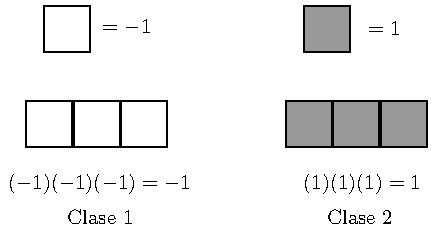
\includegraphics[scale=1.2]{redes-1.pdf} 
\caption{Patrones de entrenamiento (Datos de entrenamiento).}
\end{figure}
\begin{figure}[h!]
\center
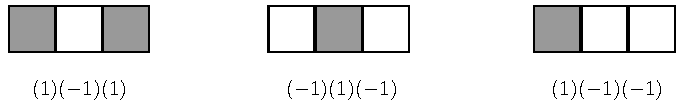
\includegraphics[scale=1.2]{redes-2.pdf} 
\caption{Datos de prueba.}
\end{figure}
\addpoints

\question[3] Sabemos de la regla de entrenamiento Delta para entrenar un Perceptron que el error cuadr\'atico medio es
\begin{equation*}
	E(\vec{w})=\frac{1}{2}\displaystyle\sum_{d\in D}(t_d-o_d)^2,
\end{equation*}
donde $D$ es el conjunto de datos de entrenamiento y la forma de actualizaci\'on del vector $\vec{w}$ esta dada por
\begin{equation*}
	\vec{w}\leftarrow \vec{w}+\Delta\vec{w},
\end{equation*}
donde $\Delta\vec{w}=-\eta\nabla E(\vec{w})$. Deducir la expresi\'on de actualizaci\'on para cada par\'ametro del vector $\vec{w}$.
\addpoints

\question[3] Considerar los datos en el espacio unidimensional mostrados en la Figura 3. Hallar el clustering \'optimo para $k=2$, iniciando con los centroides $\mu_1=2$ y $\mu_2=4$.
\begin{figure}[h!]
\center
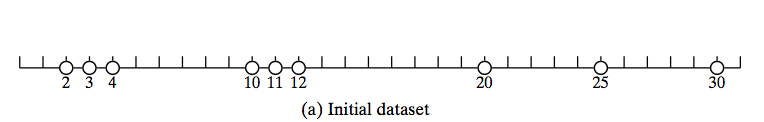
\includegraphics[scale=0.6]{ejempl1-1D-kmeans.png} 
\caption{Datos de entrenamiento Clustering.}
\end{figure}
\addpoints


\end{questions}

\end{document}
